\documentclass[12pt, titlepage]{article}

\usepackage{fullpage}
\usepackage{color}
\usepackage{ulem}
\usepackage[round]{natbib}
\usepackage{multirow}
\usepackage{booktabs}
\usepackage{tabularx}
\usepackage{graphicx}
\usepackage{float}
\usepackage{hyperref}
\hypersetup{
    colorlinks,
    citecolor=black,
    filecolor=black,
    linkcolor=red,
    urlcolor=blue
}
\usepackage[round]{natbib}

\newcounter{acnum}
\newcommand{\actheacnum}{AC\theacnum}
\newcommand{\acref}[1]{AC\ref{#1}}

\newcounter{ucnum}
\newcommand{\uctheucnum}{UC\theucnum}
\newcommand{\uref}[1]{UC\ref{#1}}

\newcounter{mnum}
\newcommand{\mthemnum}{M\themnum}
\newcommand{\mref}[1]{M\ref{#1}}

\title{SE 3XA3: Software Requirements Specification\\Asteroids War Game}

\author{Team \#12, Asteroids War Game
		\\ Eric Thai thaie1
		\\ Tianzheng Mai mait6
		\\ Junhong Chen chenj297
		\\ Linqi Jiang jiang121
}

\date{\today}


\begin{document}
\begin{table}[bp]
\centering
\caption{\bf Revision History}
\begin{tabularx}{\textwidth}{p{3cm}p{2cm}X}
\toprule {\bf Date} & {\bf Version} & {\bf Notes}\\
\midrule
March 17, 2021 & 1.0 & Section 1-4\\
March 19, 2021 & 2.0 & Section 5-7\\
March 19, 2021 & 3.0 & MIS\\
April 12, 2021 & 4.0 & Final Revision\\
\bottomrule
\end{tabularx}
\end{table}


\maketitle

\pagenumbering{roman}
\tableofcontents
\listoftables
\listoffigures


\newpage

\pagenumbering{arabic}

\section{Introduction}
\subsection{Project Overview} \label{SecAchange}
Asteroids Multiplayer is based off of the classic arcade game Asteroids with the added functionality of playing with another player. It also refactors the original code to which the user interface is greatly improved to better the game-play experience and user \sout{help} \textcolor{red}{manual} page is also added for better understanding of the game opration rules.
\subsection{Document Overview} \label{SecAchange}
This document will connect the products functional and non-functional requirements to the technical implementation details including an overview on changes to the system, a module hierarchy, connections between requirements and design, module decomposition, a trace-ability matrix and a module use hierarchy diagram.
\subsection{Document Context} \label{SecAchange}

Decomposing a system into modules is a commonly accepted approach to developing
software.  A module is a work assignment for a programmer or programming
team.  We advocate a decomposition
based on the principle of information hiding.  This
principle supports design for change, because the ``secrets'' that each module
hides represent likely future changes.  Design for change is valuable in SC,
where modifications are frequent, especially during initial development as the
solution space is explored.  

Our design follows the rules as follows:
\begin{itemize}
\item System details that are likely to change independently should be the
  secrets of separate modules.
\item Each data structure is used in only one module.
\item Any other program that requires information stored in a module's data
  structures must obtain it by calling access programs belonging to that module.
\end{itemize}

After completing the first stage of the design, the Software Requirements
Specification (SRS), the Module Guide (MG) is developed. The MG
specifies the modular structure of the system and is intended to allow both
designers and maintainers to easily identify the parts of the software.  The
potential readers of this document are as follows:

\begin{itemize}
\item New project members: This document can be a guide for a new project member
  to easily understand the overall structure and quickly find the
  relevant modules they are searching for.
\item Maintainers: The hierarchical structure of the module guide improves the
  maintainers' understanding when they need to make changes to the system. It is
  important for a maintainer to update the relevant sections of the document
  after changes have been made.
\item Designers: Once the module guide has been written, it can be used to
  check for consistency, feasibility and flexibility. Designers can verify the
  system in various ways, such as consistency among modules, feasibility of the
  decomposition, and flexibility of the design.
\end{itemize}

The rest of the document is organized as follows. Section
\ref{SecChange} lists the anticipated and unlikely changes of the software
requirements. Section \ref{SecMH} summarizes the module decomposition that
was constructed according to the likely changes. Section \ref{SecConnection}
specifies the connections between the software requirements and the
modules. Section \ref{SecMD} gives a detailed description of the
modules. Section \ref{SecTM} includes two traceability matrices. One checks
the completeness of the design against the requirements provided in the SRS. The
other shows the relation between anticipated changes and the modules. Section
\ref{SecUse} describes the use relation between modules.

\section{Anticipated and Unlikely Changes} \label{SecChange}

This section lists possible changes to the system. According to the likeliness
of the change, the possible changes are classified into two
categories. Anticipated changes are listed in Section \ref{SecAchange}, and
unlikely changes are listed in Section \ref{SecUchange}.

\subsection{Anticipated Changes} \label{SecAchange}

Anticipated changes are the source of the information that is to be hidden
inside the modules. Ideally, changing one of the anticipated changes will only
require changing the one module that hides the associated decision. The approach
adapted here is called design for
change.

\begin{description}
\item[\refstepcounter{acnum} \actheacnum \label{browser}:] The web browser the software is being run on.
\item[\refstepcounter{acnum} \actheacnum \label{hardware}:] The hardware the software is being run on.
\item[\refstepcounter{acnum} \actheacnum \label{players}:] The amount of additional players that can play together.
\item[\refstepcounter{acnum} \actheacnum \label{additional features}:] Additional features such as power-ups or new enemies.
\item[\refstepcounter{acnum} \actheacnum \label{game modes}:] The different game modes being added.


\end{description}

\subsection{Unlikely Changes} \label{SecUchange}

The module design should be as general as possible. However, a general system is
more complex. Sometimes this complexity is not necessary. Fixing some design
decisions at the system architecture stage can simplify the software design. If
these decision should later need to be changed, then many parts of the design
will potentially need to be modified. Hence, it is not intended that these
decisions will be changed.

\begin{description}
\item[\refstepcounter{ucnum} \uctheucnum \label{ucIO}:] Input and output devices (standard keyboard and monitor) are unlikely to change.
\item[\refstepcounter{ucnum} \uctheucnum \label{ucInput}:] The core game purpose (spaceship shooting objects in space while avoiding being hit by other objects/projectiles)
\item[\refstepcounter{ucnum} \uctheucnum \label{ucInput}:] The method in which 2 players can play the game together (single device)
\end{description}

\section{Module Hierarchy} \label{SecMH}

This section provides an overview of the module design. Modules are summarized
in a hierarchy decomposed by secrets in Table \ref{TblMH}. The modules listed
below, which are leaves in the hierarchy tree, are the modules that will
actually be implemented.

\begin{description}
\item [\refstepcounter{mnum} \mthemnum \label{mHH}:] Hardware-Hiding Module
\item [\refstepcounter{mnum} \mthemnum \label{mBH}:] Behaviour-Hiding Module
\item [\refstepcounter{mnum} \mthemnum \label{mSD}:] Software Decision Module
\item [\refstepcounter{mnum} \mthemnum \label{mG}:] Game Module
\item [\refstepcounter{mnum} \mthemnum \label{mS}:] Ship Module
\item [\refstepcounter{mnum} \mthemnum \label{mGC}:] Game Canvas Module
\item [\refstepcounter{mnum} \mthemnum \label{mA}:] Asteroid Module
\item [\refstepcounter{mnum} \mthemnum \label{mM}:] Menu Module
\item [\refstepcounter{mnum} \mthemnum \label{mE}:] Alien Module
\end{description}


\begin{table}[h!]
\centering
\begin{tabular}{p{0.3\textwidth} p{0.6\textwidth}}
\toprule
\textbf{Level 1} & \textbf{Level 2}\\
\midrule

{Hardware-Hiding Module} & ~ \\
\midrule

\multirow{2}{0.3\textwidth}{Behaviour-Hiding Module}
& \mref{mG}\\
& \mref{mGC}\\
& \mref{mM}\\
\midrule

\multirow{3}{0.3\textwidth}{Software Decision Module} 
& \mref{mS}\\
& \mref{mA}\\
& \mref{mE}\\
\bottomrule

\end{tabular}
\caption{Module Hierarchy}
\label{TblMH}
\end{table}

\section{Connection Between Requirements and Design} \label{SecConnection}

The design of the system is intended to satisfy the requirements developed in
the SRS. In this stage, the system is decomposed into modules. The connection
between requirements and modules is listed in Table \ref{TblRT}.


\section{Module Decomposition} \label{SecMD}

Modules are decomposed according to the principle of ``information hiding''
. The \emph{Secrets} field in a module
decomposition is a brief statement of the design decision hidden by the
module. The \emph{Services} field specifies \emph{what} the module will do
without documenting \emph{how} to do it. For each module, a suggestion for the
implementing software is given under the \emph{Implemented By} title. If the
entry is \emph{OS}, this means that the module is provided by the operating
system or by standard programming language libraries.  Also indicate if the
module will be implemented specifically for the software.

Only the leaf modules in the
hierarchy have to be implemented. If a dash (\emph{--}) is shown, this means
that the module is not a leaf and will not have to be implemented. Whether or
not this module is implemented depends on the programming language
selected.

\subsection{Hardware Hiding Modules (\mref{mHH})}

\begin{description}
\item[Secrets:]The data structure and algorithm used to implement the virtual
  hardware.
\item[Services:]Serves as a virtual hardware used by the rest of the
  system. This module provides the interface between the hardware and the
  software. So, the system can use it to display outputs or to accept inputs.
\item[Implemented By:] OS
\end{description}

\subsection{Behaviour-Hiding Module  (\mref{mBH})}

\begin{description}
\item[Secrets:]The contents of the required behaviours.
\item[Services:]Includes programs that provide externally visible behaviour of
  the system as specified in the software requirements specification (SRS)
  documents. This module serves as a communication layer between the
  hardware-hiding module and the software decision module. The programs in this
  module will need to change if there are changes in the SRS.
\item[Implemented By:] --
\end{description}

\subsubsection{Game Module (\mref{mG})}

\begin{description}
\item[Secrets:]\sout{How the scores are calculated. How the game is loaded before playing the game.  How the game is running when playing the game.}
\textcolor{red}{The data structure and algorithm used to calculate the user's scores and implement the game.}
\item[Services:]Handles all the game logic such as algorithm of loading the game, running the game, calculating the scores, etc.
\item[Implemented By:] Asteroid project
\end{description}

\subsubsection{Game Canvas Module (\mref{mGC})}

\begin{description}
\item[Secrets:]\sout{How the game objects are drawn on the canvas. How the game is displayed on the html web page} \textcolor{red}{The data structure and algorithm used to draw the game objects and canvas onto the screen}.
\item[Services:]Displays the game board and the game objects such as background image, asteroids, spaceship, Aliens, and bullets.
\item[Implemented By:] main1.html, main2.html, game1.js, game2.js
\end{description}

\subsubsection{Menu Module  (\mref{mM})}

\begin{description}
\item[Secrets:]\sout{How the menu of the game is created. How the menu of the game is formatted and structured. How the buttons link to other web pages.} \textcolor{red}{The data structure and algorithm used to create, format and structure the main menu of the game}
\item[Services:]Displays the menu of the game, formats the text and background image of the game, and provides buttons that allow the user to go to other pages.
\item[Implemented By:] index.html
\end{description}

\subsection{Software Decision Module (\mref{mSD})}

\begin{description}
\item[Secrets:] The design decision based on mathematical theorems, physical
  facts, or programming considerations. The secrets of this module are
  \emph{not} described in the SRS.
\item[Services:] Includes data structure and algorithms used in the system that
  do not provide direct interaction with the user. 
  % Changes in these modules are more likely to be motivated by a desire to
  % improve performance than by externally imposed changes.
\item[Implemented By:] --
\end{description}

\subsubsection{Ship Module  (\mref{mS})}

\begin{description}
\item[Secrets:]\sout{How the spaceship interacts with other objects in the game, such as aliens and asteroids. How the spaceship is controlled by the player.}
\textcolor{red}{The data structure and algorithm used to implement the user's spaceship object in the game, determining how the spaceship interacts with other objects in the game, such as aliens and asteroids and how the spaceship is controlled by the player.} 
\item[Services:]Provides the functionalities of spaceship object.
\item[Implemented By:] game1.js. game2.js
\end{description}

\subsubsection{Asteroid Module  (\mref{mA})}

\begin{description}
\item[Secrets:]\sout{How the asteroids interact with other objects in the game such as aliens, spaceship and bullets. How the asteroid is broken up after a collision.}
\textcolor{red}{The data structure and algorithm used to implement the asteroid pbject in the game, determining how the asteroids interact with other objects in the game such as aliens, spaceship and bullets and how the asteroid is broken up after a collision.} 
\item[Services:]Provides the functionalities of asteroid object.
\item[Implemented By:] game1.js. game2.js
\end{description}

\subsubsection{Alien Module  (\mref{mE})}

\begin{description}
\item[Secrets:]\sout{How the alien interacts with other objects in the game such as asteroids, spaceship and bullets. How the speed and the direction of the alien object are set.}
\textcolor{red}{The data structure and algorithm used to implement the alien object in the game, determining how the alien interacts with other objects in the game such as asteroids, spaceship as well as bullets and the attributes of the alien object.} 
\item[Services:]Provides the functionalities of alien object.
\item[Implemented By:] game1.js. game2.js
\end{description}

\section{Traceability Matrix} \label{SecTM}

This section shows two traceability matrices: between the modules and the
requirements and between the modules and the anticipated changes.

% the table should use mref, the requirements should be named, use something
% like fref

\begin{table}[H]
\centering
\begin{tabular}{p{0.2\textwidth} p{0.6\textwidth}}
\toprule
\textbf{Req.} & \textbf{Modules}\\
\midrule
R1 & \mref{mHH}, \mref{mBH}, \mref{mSD} \\
R2 & \mref{mG}, \mref{mGC}\\
R3 & \mref{mG}, \mref{mS},\mref{mGC}, \mref{mA}, \mref{mE}\\
R4 & \mref{mBH}, \mref{mG}, \mref{mGC}\\
R5 & \mref{mG}, \mref{mGC}, \mref{mA}, \mref{mE}\\
R6 & \mref{mHH}, \mref{mBH}, \mref{mSD}, \mref{mG}, \mref{mS}, \mref{mGC}\\
R7 & \mref{mM}\\
R8 & \mref{mG}, \mref{mGC}\\
R9 & \mref{mS}, \mref{mG},\mref{mGC}\\
\textcolor{red}{R10} & \textcolor{red}{\mref{mM}}\\
\textcolor{red}{R11} & \textcolor{red}{\mref{mS}, \mref{mG},\mref{mGC}}\\
\bottomrule
\end{tabular}
\caption{Trace Between Requirements and Modules}
\label{TblRT}
\end{table}
\begin{table}[H]
\centering
\begin{tabular}{p{0.2\textwidth} p{0.6\textwidth}}
\toprule
\textbf{AC} & \textbf{Modules}\\
\midrule
\acref{browser} &\mref{mGC}\\
\acref{hardware} & \mref{mHH}\\
\acref{players} & \mref{mG},\mref{mS} \\
\acref{additional features} & \mref{mBH},\mref{mG}, \mref{mGC},\mref{mSD}\\
\acref{game modes} &\mref{mG},\mref{mA}, \mref{mE}\\
\bottomrule
\end{tabular}
\caption{Trace Between Anticipated Changes and Modules}
\label{TblACT}
\end{table}

\section{Use Hierarchy Between Modules} \label{SecUse}

In this section, the uses hierarchy between modules is
provided. Two programs A and B that A {\em uses} B if
correct execution of B may be necessary for A to complete the task described in
its specification. That is, A {\em uses} B if there exist situations in which
the correct functioning of A depends upon the availability of a correct
implementation of B.  Figure \ref{FigUH} illustrates the use relation between
the modules. It can be seen that the graph is a directed acyclic graph
(DAG). Each level of the hierarchy offers a testable and usable subset of the
system, and modules in the higher level of the hierarchy are essentially simpler
because they use modules from the lower levels.

\begin{figure}[H]
\centering
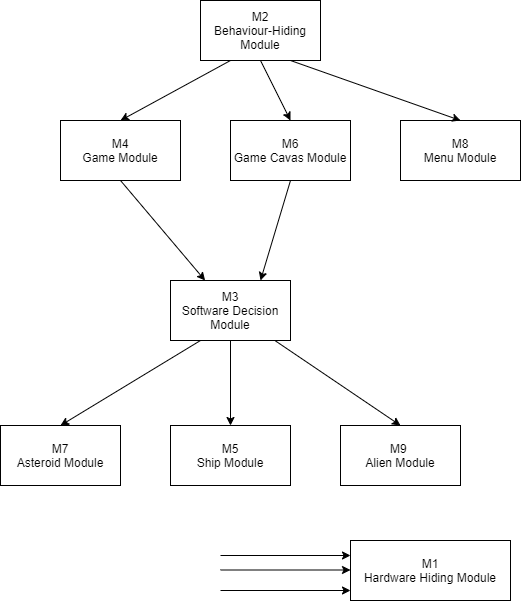
\includegraphics[width=0.7\textwidth]{modules.png}
\caption{Use hierarchy among modules}
\label{FigUH}
\end{figure}

%\section*{References}

\bibliographystyle {plainnat}
\bibliography {MG}

\end{document}
